\section{L'organisation spatiale des espèces, histroire et espoir}

\section{Interactions et biogéographie}

% \begin{sloppypar} [De façon générale, la thèse ou le mémoire sous forme d’articles comporte une introduction générale, autant de chapitres qu’il y a d’articles, une conclusion générale et une liste des références bibliographiques, qui peut être globale ou par article. Dans ce cas, il faut aussi inclure à la fin une liste des références bibliographiques pour l’introduction et la conclusion.
%
% L’introduction générale doit présenter la problématique des travaux de recherche, les principales dimensions méthodologiques, s'il y a lieu, et les résultats obtenus directement en rapport avec la contribution de celui qui produit la thèse ou le mémoire. Il faut bien montrer comment se situe la contribution originale de l'auteur (ou des auteurs) par rapport aux travaux cités dans la liste des références bibliographiques. Les sous-titres de l’introduction générale ne sont pas numérotés.
%
% L'étudiant n'a pas à exposer en introduction ce qui le sera en détails dans les articles. Il peut par contre s’y référer pour appuyer les points abordés.
% L’insertion d’articles dans un mémoire ou une thèse doit se faire dans le respect le plus strict du droit d’auteur. De plus, l'étudiant qui présente un mémoire ou une thèse sous forme d’articles doit s'assurer, avant le dépôt final de son document, de l'obtention des droits de reproduction de ces articles s'ils sont déjà publiés ou à paraître.
%
% L'étudiant assume l'entière responsabilité de l'écriture et de la présentation de la version finale du rapport qu'il rédige dans le cadre de son programme d'études. Pour plus ample information concernant les droits d’auteur, pour prendre connaissance des questions courantes sur le sujet ou pour consulter Le guide des droits d’auteur de l’Office de la propriété intellectuelle du Canada, cliquer sur le lien suivant : \url{http://www.opic.ic.gc.ca/eic/site/cipointernet-internetopic.nsf/fra/h_wr02281.html}
%
% Pour consulter la Politique sur la reconnaissance et la protection de la propriété intellectuelle de l’UQAR, cliquer sur le lien suivant : \url{http://www.uqar.ca/files/secretariat-general/politiques/enseignement-recherche/37c2.pdf}
%
% L’information présentée dans les chapitres suivants est exposée de façon à fournir un exemple de division de chapitres et de sections.] \end{sloppypar}
%
% \section*{Modalités de pagination} % L'étoile est là pour éviter la numérotation de la section
% \addcontentsline{toc}{section}{\protect\numberline{}Modalités de pagination} % Cette commande sert à ajouter le titre dans la table des matières malgré l'absence de numérotation
%
% [Toutes les pages du texte, à l’exception des pages de garde, comptent dans la pagination. Mises à part les pages titres, les pages liminaires (précédent l’introduction) sont paginées en \textbf{chiffres romains minuscules}. Avec l’introduction, débute la pagination en \textbf{chiffres arabes} (en commençant à 1) y compris pour les pages comportant des tableaux, des graphiques, des schémas, des dessins ainsi que les appendices, les annexes et les index, s'il y a lieu.
%
% Ainsi, la page de titre du document est la page i (un) non paginée, alors que la page de titre de l’introduction est la page 1 (un) comptée mais non paginée. Enfin, la page qui contient un tableau (ou une figure) et qui est orienté dans le sens opposé (orientation de type paysage) est comptée, mais non paginée.
%
% Le positionnement des \textbf{pages amorçant des débuts de section ou de chapitre} est toujours à droite (recto) en page impaire. Les pages de gauche (verso) portent toujours un nombre pair. Si un chapitre finit en page de droite, on insère une page blanche (insérée automatiquement lors de l’impression grâce au saut de section « Page impaire » et comptée dans la numérotation) avant de commencer un nouveau chapitre. Le positionnement du numéro de page en haut à droite s’appliquera aux pages impaires, réalisées en recto. Le numéro de page, \textbf{sans point ni tiret}, devra apparaître en haut à gauche pour les pages paires, en verso. En aucun cas, des points de suspension ou un trait oblique en bas de page ne doivent apparaître.]
%
% \section*{Modalités de présentation des tableaux}
% \addcontentsline{toc}{section}{\protect\numberline{}Modalités de présentation des tableaux}
%
% Les tableaux doivent être identifiés par un titre situé au-dessus et numérotés en chiffres arabes. Le titre ne doit pas excéder la largeur du tableau. Lorsqu’un élément du tableau requiert une explication additionnelle, un appel de note (lettre ou astérisque) peut être inséré à l’endroit où l’explication est requise. La note explicative est présentée sous le tableau (voir tableau 1). Lorsque la source du tableau est citée, cette dernière est placée après la note explicative et l’information est alignée sur la marge de gauche.
%
% \begin{table}[h]
% 	\renewcommand{\arraystretch}{0.75}
% 	\caption{Titre \textbf{court et précis} du premier tableau}
% 	\newcolumntype{Y}{>{\raggedright\arraybackslash}X}
% 	{\begin{tabularx}{\linewidth}{YYYYY} \toprule
% 	& \textbf{Facteur A} & \textbf{Facteur B} & \textbf{Facteur C} & \textbf{Facteur D} \\ \midrule
% 	\textbf{Segment A} & & & & \\ \addlinespace
% 	\textbf{Segment B\textsuperscript{*}} & & & & \\ \addlinespace
% 	\textbf{Segment C} & & & & \\ \addlinespace
% 	\textbf{Segment D} & & & & \\ \addlinespace
% 	\bottomrule
% 	\end{tabularx}}
% 	\newline \textsuperscript{*}Ceci est une explication additionnelle concernant le segment B.
% 	\newline Source : \textit{Le guide alimentaire canadien}, 2009. Santé Canada.
% \end{table}
%
% \section*{Modalités de présentation des figures}
% \addcontentsline{toc}{section}{\protect\numberline{}Modalités de présentation des figures}
%
% Les figures (graphique, schéma, croquis, photographie, diagramme, et toute autre illustration) doivent être centrées par rapport au texte en respectant les instructions de mise en page. Chaque figure est numérotée en chiffres arabes. Le titre, en minuscule, doit être court et précis (sans point final) et est placé sous l'illustration et à gauche (voir figure 1). Lorsque c'est le cas, indiquer la ou les sources d'où provient l'information.
%
% \afterpage{
% \begin{figure}
% 	\centering
%     \captionbox
%     {Titre \textbf{court et précis} de la première figure}
%     {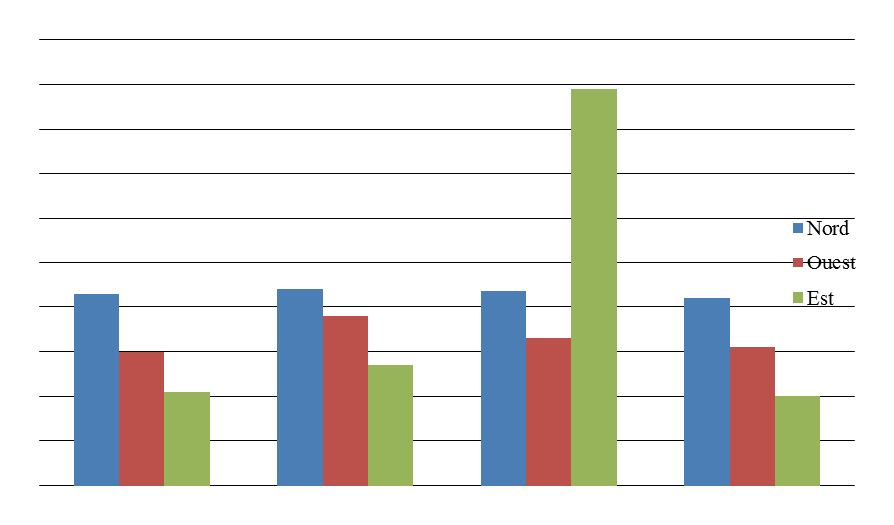
\includegraphics[width=30pc]{figure_exemple}}
% \end{figure}
% }
